% !Mode:: "TeX:UTF-8"
% Author: Zhengxi Tian
% Email: zhengxi.tian@hotmail.com

\chapter{相关工作}\label{ch:related_work}
\section{生成式模型}\label{sec:generative_model}
一个生成式模型定义了给定输入序列$X = x_1, x_2, \cdots, x_n$,
任意输出序列$Y = y_1, y_2, \cdots, y_m$的条件概率$p(Y|X)$。
模型的训练目标就是在数据集$S$上最大化给定$X$,$Y$的对数概率(Log Probability):
\begin{align}
    \mathit{L} = \frac{1}{|S|} \sum_{(Y, X) \in S} \log p(Y|X)
\end{align}
从这个角度来看,语言模型\upcite{
    DBLP:journals/jmlr/BengioDVJ03,
    DBLP:conf/interspeech/MikolovKBCK10}(Language Model)和编解码器都属于生成式模型,
因为它们都定义了条件概率$p(Y|X)$。不管什么样的实现,生成式模型都要解决对序列建模的问题,
即把一个长度可变的序列$X$映射到另一个长度可变的序列$Y$,且$X$和$Y$的长度可以不相等。
循环神经网络(RNN)为这个问题提供了天然的解决方案。
% 介绍RNN,unrolled
RNN的基本思想是,序列由有序的元素组成,每一个元素用一个时刻(Time Step)来描述,
在某一个时刻$t_i$,RNN接受输入序列$X$中的某个元素$x_i$,并输出一个元素$y_i$;
在下一个时刻$t_{i+1}$,RNN接受输入元素$x_{i+1}$,并输出一个元素$y_{i+1}$。
让RNN与普通神经网络不同的是,RNN在一系列时刻的输入输出中不断更新同一个权重矩阵$W_{h}$,
它又被称为循环矩阵(Recurrent Matrix)。
循环矩阵的作用是记忆输入序列的位置信息,并把当前时刻的输入序列编码成一个定长向量。
图~\ref{fig:RNN_unrolled}\footnote{http://colah.github.io/posts/2015-08-Understanding-LSTMs/}
描述了简化的RNN结构。
\begin{figure}[H]
    \centering
    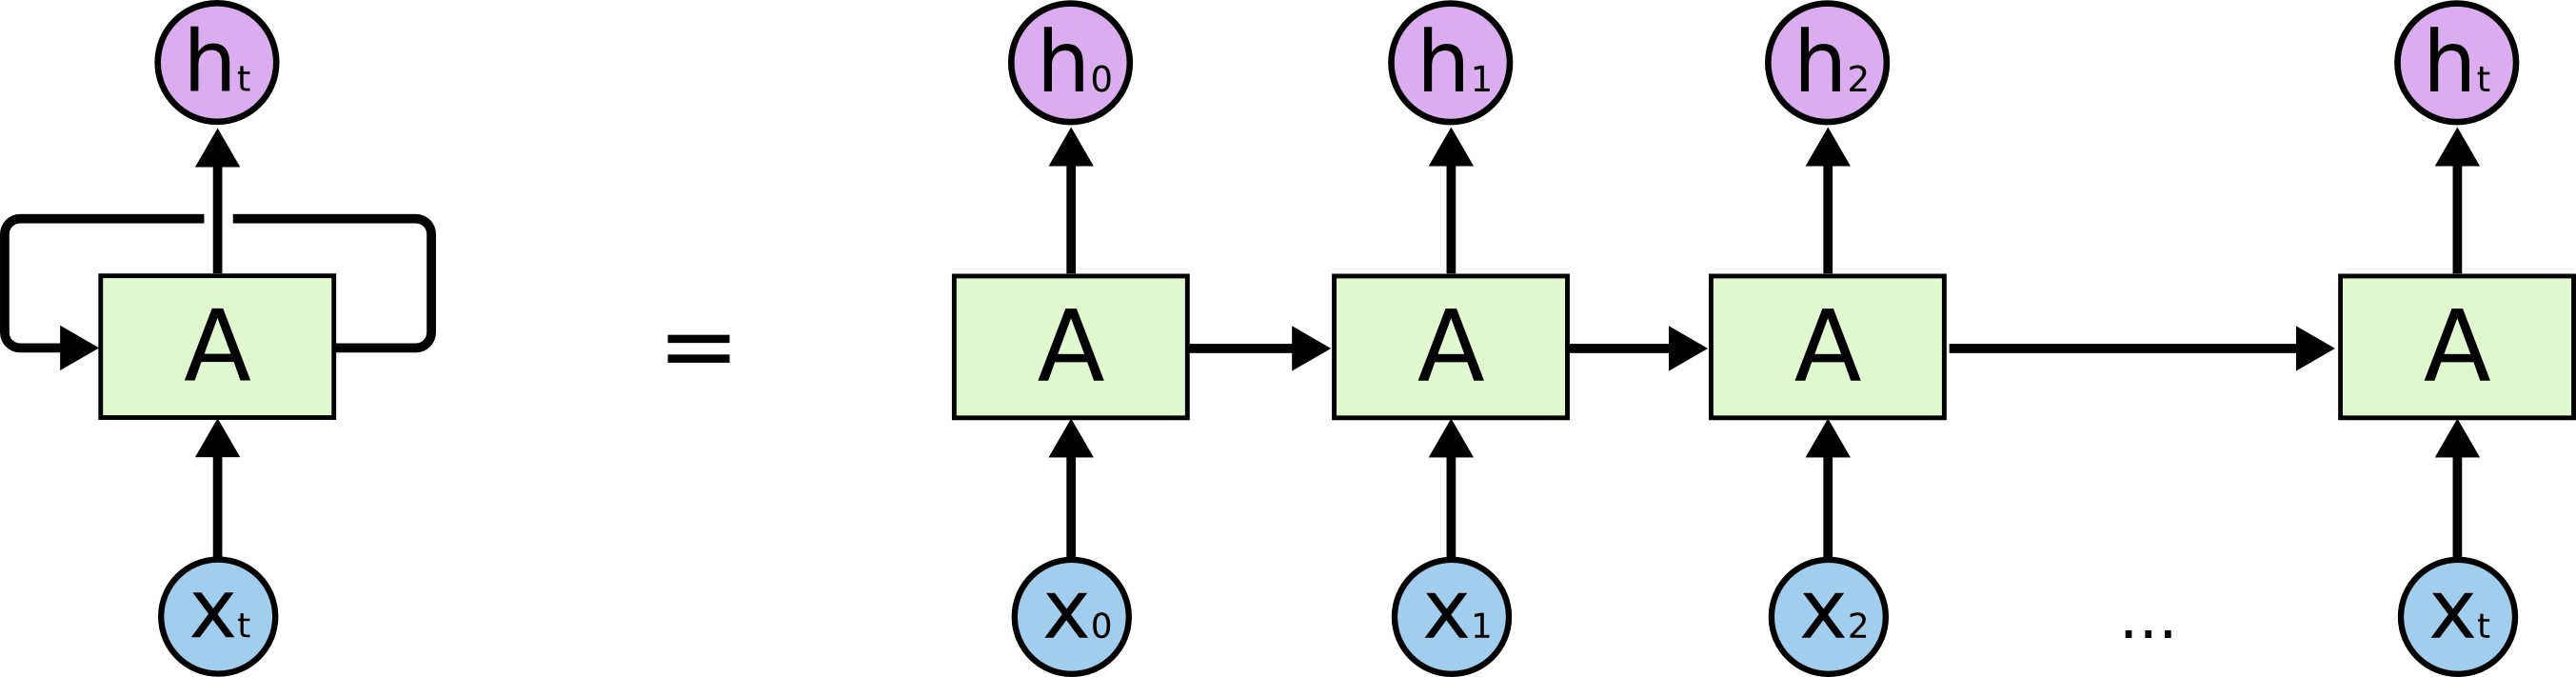
\includegraphics[width=0.6\textwidth]{figure/RNN-unrolled.png}
    \caption{RNN的一般表示和展开表示}
    \label{fig:RNN_unrolled}
\end{figure}

\section{自动化评价指标}\label{sec:automatic_metric}

\section{公开的对话数据集}\label{sec:public_dataset}

\section{本章小结}\label{sec:rw_conclusion}
%这一节总结所有提及的指标,给它们分一下类,然后简要说明每一类
%指标的特点,或者是它考察的方面。
